In order to verify and validate the design, each module are tested and compared with simulation results. The corresponding tests verifies the feasibility of the design.

The measurement of the clock generator and a phase of the RF field (RF+) is shown in the Fig. \ref{fig:meas}.a. The wave demonstrates that the CG works well and can divide the clock 13.56MHz/4. The ripple of the clock is due to the noise of external power source which the ring pad is connected. 

Fig. \ref{fig:meas}.b shows the comparison between RF+ with the output of the POR module. It can be seen the delay of the POR in relation to the input signal. This delay allows the DPU changing to the idle state.

Finally, Fig. \ref{fig:meas}.c shows the signal recovery transmitted from PCD. It demonstrates that the clock is interrupted, when a frame arrives.

\begin{figure}[h]
  \centering
  \includegraphics[page=20,width=80mm]{images-crop.pdf}
  \caption{(a) Clk/4 vs RF+, (b) RF+ vs POR, (c) Clk/4 vs Demodulator}
  \label{fig:meas}
\end{figure}